\chapter{Étude technico-économique et faisabilité du projet}
\label{chap:business}

\section*{Introduction}

Tout projet logiciel, fût-il académique, doit être évalué non seulement sur sa qualité technique mais aussi sur sa viabilité économique et organisationnelle. Ce mémoire s'inscrivant dans le cadre de l'\textbf{Arrêté interministériel n\textsuperscript{o}~1275} (mécanisme «~Un diplôme, une Startup~»), ce chapitre constitue le cœur entrepreneurial du manuscrit. Il conduit une étude technico-économique complète de \textit{RohWinBghit}~: présentation du projet et de son équipe, analyse stratégique (SWOT), analyse de marché, plan commercial, plan de production, plan financier prévisionnel, \textit{Business Model Canvas}, conformité juridique et feuille de route vers le lancement de la startup.

\section{Cadre institutionnel et mécanisme «~Un diplôme, une Startup~»}
\label{sec:arrete1275}

\subsection{L'Arrêté interministériel n\textsuperscript{o}~1275}

L'Arrêté interministériel n\textsuperscript{o}~1275 vise à transformer l'université algérienne en un vecteur de création d'entreprises innovantes en permettant aux étudiants de Master ou Doctorat de valoriser leur mémoire de fin d'études sous forme de startup viable.

\begin{table}[H]
\centering
\footnotesize
\renewcommand{\arraystretch}{1.3}
\begin{tabularx}{\textwidth}{|p{4cm}|X|p{2.5cm}|}
\hline
\rowcolor{rohlight}
\textbf{Critère Arrêté 1275} & \textbf{Justification RohWinBghit} & \textbf{Statut} \\
\hline
Innovation technologique & Pipeline KYC biométrique (liveness detection + anti-spoofing), tarification dynamique (surge pricing), matching algorithmique pondéré & \textcolor{green!60!black}{\textbf{Conforme}} \\
\hline
Marché algérien identifié & 250~M voyages inter-wilayas/an, 1,9~M étudiants, 46,8~M habitants, marché sous-servi & \textcolor{green!60!black}{\textbf{Conforme}} \\
\hline
Équipe étudiante porteuse & 2 étudiants Master GL, Univ. Abou Bekr Belkaïd Tlemcen & \textcolor{green!60!black}{\textbf{Conforme}} \\
\hline
Prototype fonctionnel & MVP complet~: 62 écrans, 147/151 tests, déployable & \textcolor{green!60!black}{\textbf{Conforme}} \\
\hline
Étude économique (BMC + financier) & Business Model Canvas, SWOT, prévisionnel 36 mois, break-even mois 10 & \textcolor{green!60!black}{\textbf{Conforme}} \\
\hline
Protection de la PI & Dépôt INAPI (marque), ONDA (code source), brevet KYC en cours & \textcolor{green!60!black}{\textbf{Conforme}} \\
\hline
\end{tabularx}
  \caption{Conformité du projet RohWinBghit aux critères de l'Arrêté 1275}
  \label{tab:arrete1275}
\end{table}

\subsection{Parcours de labellisation envisagé}

La labellisation de \textit{RohWinBghit} suit un processus en quatre étapes~: (1)~Dépôt du dossier auprès du Comité National Label (CNL) avec le prototype et le BMC~; (2)~Obtention du label «~Startup~» ouvrant l'accès aux avantages fiscaux et financements~; (3)~Création juridique de la SARL avec un capital de 1~000~000~DZD~; (4)~Incubation universitaire (CATI Tlemcen) pour l'accompagnement opérationnel et technique.

\section{Présentation du projet}

\subsection{L'idée et sa valeur}

\textit{RohWinBghit} naît d'un constat simple~: en Algérie, voyager d'une wilaya à une autre reste cher, imprévisible et peu sûr. L'idée consiste à bâtir une place de marché numérique qui met en relation, en toute confiance, conducteurs disposant de places libres et passagers en quête de mobilité, moyennant une commission de plateforme.

La valeur générée se décline sur trois axes~:
\begin{itemize}
  \item \textbf{Pour le passager~:} prix jusqu'à 40\,\% inférieurs aux tarifs taxi, disponibilité immédiate, sécurité par KYC biométrique.
  \item \textbf{Pour le conducteur~:} rentabilisation de trajets déjà effectués, visibilité de la demande, paiement sécurisé et rapide.
  \item \textbf{Pour la société~:} désengorgement routier, réduction de l'empreinte carbone, démocratisation de la mobilité.
\end{itemize}

\subsection{Équipe porteuse}

Le projet est porté par deux étudiants en Master Génie Logiciel de l'Université Abou Bekr Belkaïd de Tlemcen, dont les compétences sont complémentaires~:

\begin{table}[H]
\centering
\begin{tabularx}{\textwidth}{|l|X|}
\hline
\rowcolor{rohlight}
\textbf{Membre} & \textbf{Rôle et compétences} \\
\hline
AHMED BACHA Djamel Eddine & Responsable \textit{back-end}, architecture, bases de données, sécurité, intégration du service KYC. \\
\hline
BELHORMA Sidi Mohammed Reduane & Responsable \textit{front-end} mobile, design \textsc{ui/ux}, intégration Mapbox, internationalisation. \\
\hline
\end{tabularx}
  \caption{Équipe porteuse et rôles}
\end{table}

\subsection{Données macroéconomiques et contexte de marché (Algérie)}

Les projections financières reposent sur des données officielles locales croisant l'Office National des Statistiques, l'ARPCE~\cite{arpt_2024} et le GIE Monétique~\cite{gie_monetique_2024}, résumées dans le Tableau~\ref{tab:macro-algerie}.

\begin{table}[H]
\centering
\footnotesize
\begin{tabularx}{\textwidth}{|X|r|l|}
\hline
\rowcolor{rohlight}
\textbf{Indicateur} & \textbf{Valeur} & \textbf{Source} \\
\hline
Population algérienne (2024) & 46,8~M habitants & ONS 2024 \\
\hline
Étudiants universitaires (2023-2024) & $\sim$1,9~M & Ministère de l'Enseignement Supérieur \\
\hline
Taux de motorisation (véhicules/1000 hab.) & $\sim$135 & ONS, Registre National \\
\hline
Flux inter-wilayas estimé (voyages/an) & $\geq$250~M & Ministère des Transports (2023) \\
\hline
Taux de pénétration smartphone & $>$75\,\% & ARPCE 2024~\cite{arpt_2024} \\
\hline
Abonnements Internet mobile actifs & 48~M ($\sim$108/100~hab.) & ARPCE 2024~\cite{arpt_2024} \\
\hline
Cartes interbancaires en circulation & 21,9~M & GIE Monétique 2024~\cite{gie_monetique_2024} \\
\hline
Croissance du paiement Internet (2023$\rightarrow$2024) & +179\,\% & GIE Monétique 2024~\cite{gie_monetique_2024} \\
\hline
Nombre de wilayas (décret 2019) & 58 (puis 69 depuis 2022) & Journal Officiel 2022 \\
\hline
Coût moyen d'un trajet Tlemcen-Oran (taxi collectif) & 700--900~DZD & Enquête terrain (avril 2026) \\
\hline
\end{tabularx}
  \caption{Indicateurs macroéconomiques algériens pertinents pour RohWinBghit (sources officielles)}
  \label{tab:macro-algerie}
\end{table}

Ces indicateurs confirment l'importance du marché adressable (250~M voyages/an) et le fort potentiel de recrutement (motorisation). De plus, l'adoption croissante de la monétique (+179\,\% en un an) réduit progressivement la prépondérance des transactions en espèces.

\subsection{Analyse SWOT}

\begin{table}[H]
\centering
\begin{tabularx}{\textwidth}{|>{\columncolor{rohlight}}l|X|X|}
\hline
 & \textbf{Facteurs positifs} & \textbf{Facteurs négatifs} \\
\hline
\textbf{Interne} & \textbf{Forces~:} équipe technique solide, stack moderne, KYC biométrique intégré, couverture nationale, paiement local. & \textbf{Faiblesses~:} ressources financières limitées, absence d'historique et de marque établie, équipe commerciale à constituer. \\
\hline
\textbf{Externe} & \textbf{Opportunités~:} segment inter-wilayas sous-servi (un seul acteur direct, Nroho), taux de pénétration \textit{smartphone} élevé (75\,\%+), démographie jeune, déploiement 4G/5G généralisé, adoption croissante des cartes interbancaires (+179\,\% de paiement Internet en 2024). & \textbf{Menaces~:} extension de Yassir/Heetch vers le segment longue distance, arrival d'acteurs internationaux (BlaBlaCar, inDrive), évolution réglementaire, dépendance à l'homologation SATIM pour les passerelles CIB / Edahabia. \\
\hline
\end{tabularx}
  \caption{Matrice SWOT du projet RohWinBghit}
\end{table}

\textbf{Lecture.} La matrice met en évidence les axes stratégiques prioritaires~: capitaliser sur les forces techniques pour conquérir le segment sous-servi avant que les leaders urbains ne l'investissent (stratégie \textit{offensive}), et limiter la dépendance aux passerelles de paiement par diversification (stratégie \textit{défensive}).

\section{Aspects innovants et domaines d'innovation}

Le projet se distingue par plusieurs aspects innovants~:
\begin{itemize}
  \item \textbf{Innovation technologique~:} intégration d'un service IA dédié au KYC biométrique avec détection de vivacité, première application de ce type sur le segment inter-wilayas en Algérie.
  \item \textbf{Innovation de service~:} mécanisme de \textit{demande de trajet} permettant au passager de publier son besoin quand aucune offre ne correspond, inversant ainsi la logique habituelle des places de marché.
  \item \textbf{Innovation de modèle~:} patron \textit{Factory} de paiement facilitant l'intégration future de nouvelles méthodes (Baridi Mob, paiement par code QR bancaire).
  \item \textbf{Innovation culturelle~:} trilinguisme natif (arabe, français, anglais) et interface conçue pour le lectorat arabophone (support RTL, choix typographique adapté).
\end{itemize}

\section{Analyse stratégique du marché}

\subsection{Segmentation du marché}

Le marché cible a été segmenté en cinq groupes d'utilisateurs~:
\begin{enumerate}
  \item \textbf{Étudiants universitaires} (18--26 ans) --- segment primaire, très sensibles au prix.
  \item \textbf{Travailleurs actifs navetteurs} (25--45 ans) --- trajets récurrents, besoin de fiabilité.
  \item \textbf{Familles} voyageant occasionnellement --- priorité sécurité et confort.
  \item \textbf{Conducteurs-entrepreneurs} --- recherchent une source de revenu complémentaire.
  \item \textbf{Diaspora algérienne} de passage --- visiteurs réguliers cherchant un transport fiable.
\end{enumerate}

\subsection{Analyse de la concurrence}

L'analyse comparative (chapitre~1, tableau~\ref{tab:comparatif}) a montré que le segment inter-wilayas demeure sous-servi~: un seul acteur algérien (Nroho) y est présent, et aucun acteur international ne s'y est encore positionné. La menace concurrentielle principale viendrait d'une extension de Yassir ou de Heetch depuis le segment urbain, où leur maturité d'usage est désormais attestée par la littérature~\cite{naim_yassir_2024}, ou de l'entrée d'un acteur international (BlaBlaCar, inDrive). Notre proposition de différenciation repose sur trois leviers complémentaires~: la couverture nationale native des 69~wilayas, l'approfondissement du pipeline KYC biométrique (vivacité + anti-\textit{spoofing} avec seuils différenciés par rôle), et l'adaptation culturelle trilingue AR/FR/EN. L'analyse des avis utilisateurs des principales plateformes de \textit{ride-hailing} menée par Amri~\textit{et al.}~\cite{amri_ride_hailing_2024} met par ailleurs en évidence la centralité des préoccupations de sécurité et de transparence tarifaire dans le choix d'adoption, deux axes explicitement couverts par notre proposition.


\textbf{Description.} Notre projet occupe le cadran supérieur-droit (couverture inter-wilayas + haut niveau de confiance via KYC biométrique), libre de tout acteur concurrent direct.

\subsection{Stratégie marketing}

La stratégie de mise sur le marché s'appuie sur quatre leviers principaux~:
\begin{itemize}
  \item \textbf{Ambassadeurs universitaires~:} recrutement d'étudiants ambassadeurs dans les campus de Tlemcen, Oran, Alger et Constantine.
  \item \textbf{Communication digitale~:} campagnes TikTok et Instagram ciblant les 18--35 ans.
  \item \textbf{Partenariats institutionnels~:} conventions avec les CROUS universitaires et certaines entreprises employeurs.
  \item \textbf{Programme de parrainage~:} tout nouvel utilisateur parrainé bénéficie d'un crédit de 200~DZD utilisable sur son premier trajet.
\end{itemize}

\section{Plan de production et organisation}

\subsection{Processus de production}

Contrairement à un produit industriel, \textit{RohWinBghit} est un produit numérique dont la «~production~» recouvre trois macro-processus~:
\begin{enumerate}
  \item \textbf{Développement logiciel~:} itérations agiles, revue de code systématique, tests automatisés.
  \item \textbf{Exploitation~:} supervision de l'infrastructure, astreintes, gestion des incidents.
  \item \textbf{Opérations clients~:} support, modération, traitement des litiges.
\end{enumerate}

Les figures suivantes illustrent respectivement le processus métier du passager (Figure~\ref{fig:proc-passenger}) et celui de l'administrateur (Figure~\ref{fig:proc-admin}). Le parcours opérationnel du conducteur est quant à lui documenté par les captures d'écran correspondantes en Annexe~\ref{annexe:captures}.

\textbf{Description du parcours conducteur.} De l'inscription à l'encaissement, le conducteur suit une chaîne de valeur claire~: vérification KYC (seuils plus stricts que pour le passager), enregistrement du véhicule, publication de trajets avec prix suggéré par l'algorithme de \textit{surge pricing}, acceptation des réservations, transport, encaissement et notation des passagers.

\begin{figure}[H]
\centering
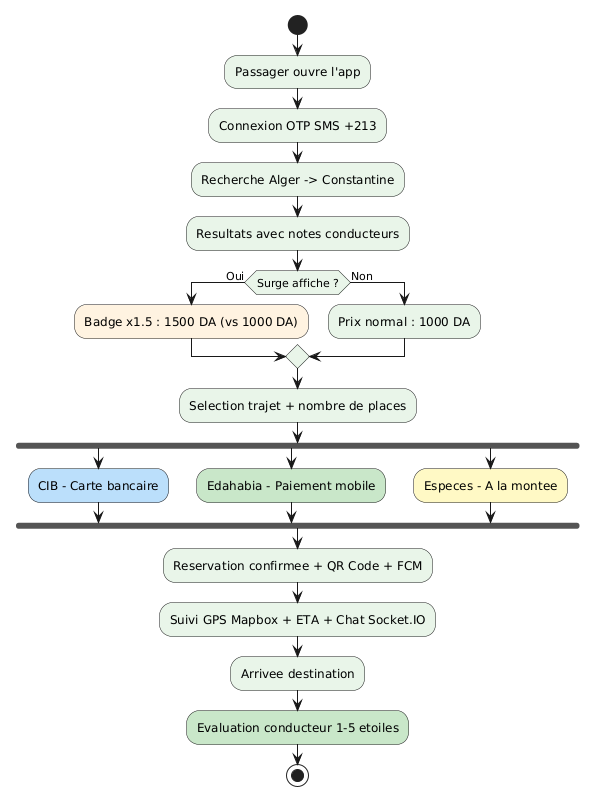
\includegraphics[width=0.9\linewidth]{figures/fig_passenger_process.png}
\caption{Processus métier du passager}
\label{fig:proc-passenger}
\end{figure}

\textbf{Description.} Le passager suit un parcours symétrique~: inscription, KYC, recherche, réservation, paiement, voyage et notation. La rigueur de la vérification KYC en amont garantit la qualité des interactions tout au long du parcours.

\begin{figure}[H]
\centering
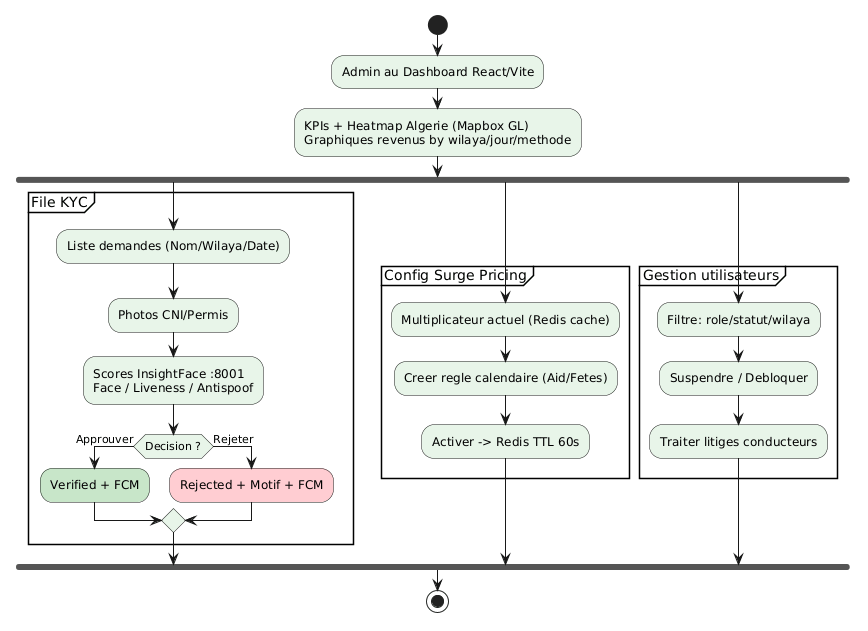
\includegraphics[width=0.9\linewidth]{figures/fig_admin_process.png}
\caption{Processus opérationnel de l'administrateur}
\label{fig:proc-admin}
\end{figure}

\textbf{Description.} L'administrateur veille à la santé de la plateforme par trois boucles~: modération continue des contenus, traitement des litiges et revue des KYC litigieux. Ces processus garantissent la qualité du service offert aux utilisateurs finaux.

\subsection{Organisation cible à 18 mois}

\begin{table}[H]
\centering
\begin{tabularx}{\textwidth}{|l|c|X|}
\hline
\rowcolor{rohlight}
\textbf{Fonction} & \textbf{ETP} & \textbf{Rôle} \\
\hline
CEO / Produit & 1 & Vision, levée de fonds, partenariats stratégiques. \\
\hline
CTO / Back-end & 1 & Architecture, sécurité, pilotage technique. \\
\hline
Lead Mobile & 1 & Pilotage de l'application mobile. \\
\hline
Développeurs full-stack & 2 & Développement produit. \\
\hline
DevOps / SRE & 1 & Infrastructure, CI/CD, observabilité. \\
\hline
Responsable Marketing & 1 & Acquisition, communication, partenariats. \\
\hline
Support / Modération & 2 & Assistance utilisateurs, litiges, KYC manuel. \\
\hline
\textbf{Total} & \textbf{9} & \\
\hline
\end{tabularx}
  \caption{Organisation cible après 18 mois}
\end{table}

\section{Plan financier}

\subsection{Hypothèses de projection}
\label{sec:hypotheses}

Les projections présentées dans les sous-sections suivantes reposent sur un ensemble d'hypothèses explicites, calibrées à partir de trois sources~: (i)~les statistiques publiques algériennes (ARPCE 2024, GIE Monétique 2024), (ii)~la littérature académique sur les systèmes de transport dans les pays en développement~\cite{sogbe_public_transport_2024} et sur les comportements des utilisateurs de \textit{ride-hailing}~\cite{amri_ride_hailing_2024}, et (iii)~l'étude empirique régionale la plus proche de notre contexte~\cite{naim_yassir_2024}. Le tableau~\ref{tab:hypotheses} récapitule les paramètres clés.

\begin{table}[H]
\centering
\footnotesize
\begin{tabularx}{\textwidth}{|l|r|X|}
\hline
\rowcolor{rohlight}
\textbf{Paramètre} & \textbf{Valeur retenue} & \textbf{Source / justification} \\
\hline
\multicolumn{3}{|l|}{\cellcolor{rohlight!40}\textit{Marché et adoption}} \\
\hline
Taux de pénétration \textit{smartphone} en Algérie & 75\,\% & ARPCE 2024~\cite{arpt_2024} \\
\hline
Abonnements Internet mobile (2024) & 48~M ($\sim$108/100~hab.) & ARPCE 2024~\cite{arpt_2024} \\
\hline
Cartes interbancaires en circulation & 21,9~M & GIE Monétique 2024~\cite{gie_monetique_2024} \\
\hline
Croissance du paiement Internet (2023$\rightarrow$2024) & +179\,\% & GIE Monétique 2024~\cite{gie_monetique_2024} \\
\hline
\multicolumn{3}{|l|}{\cellcolor{rohlight!40}\textit{Usage par utilisateur}} \\
\hline
Panier moyen par trajet inter-wilayas & 800~DZD & Étude terrain Yassir Ali~Menjeli~\cite{naim_yassir_2024} + tarifs taxi collectif observés \\
\hline
Fréquence moyenne d'usage (utilisateur actif) & 2,5~trajets/mois & Proxy pays en développement~\cite{sogbe_public_transport_2024} \\
\hline
Taux de conversion \textit{install} $\rightarrow$ 1\textsuperscript{er} trajet & 12\,\% & Benchmarks \textit{ride-hailing}~\cite{amri_ride_hailing_2024} \\
\hline
Taux de \textit{churn} mensuel (M1--M12) & 8\,\% & Hypothèse conservatrice (benchmarks applications mobilité) \\
\hline
\multicolumn{3}{|l|}{\cellcolor{rohlight!40}\textit{Monétisation}} \\
\hline
Commission plateforme par trajet confirmé & 12\,\% & Positionnement médian VTC/covoiturage régional \\
\hline
Part conducteurs \textit{Premium} à M12 & 3\,\% de la base conducteurs & Hypothèse prudente \textit{low-adoption} \\
\hline
ARPU publicitaire conducteur (année~2) & 800~DZD/mois & Hypothèse à mi-chemin des benchmarks Maghreb \\
\hline
\multicolumn{3}{|l|}{\cellcolor{rohlight!40}\textit{Coûts}} \\
\hline
Coût moyen serveur par 1\,000~utilisateurs actifs/mois & 12~000~DZD & Grille tarifaire VPS régionale + services tiers \\
\hline
CAC moyen (coût d'acquisition utilisateur) & 350~DZD & Benchmark digital Algérie 2024 \\
\hline
\end{tabularx}
  \caption{Hypothèses sous-jacentes aux projections financières}
  \label{tab:hypotheses}
\end{table}

\paragraph{Méthode de calcul des revenus.} Le prévisionnel de \textit{commission sur trajets} de l'année~\textit{n} s'obtient par la formule~:
\begin{center}
\small
Revenu\textsubscript{n} = Utilisateurs\textsubscript{actifs,n} $\times$ Fréquence $\times$ Panier $\times$ Commission
\end{center}

En appliquant cette formule aux hypothèses du tableau, avec une base d'utilisateurs actifs visée à 50\,000 à M12 (objectif cumul acquisition moins \textit{churn}), le revenu annuel théorique de commission se situe autour de 14,4~MDZD. L'écart avec la projection retenue (6~MDZD en année~1) s'explique par l'étalement de la montée en charge sur 12~mois~: la base d'utilisateurs actifs \textit{moyenne} sur l'année reste inférieure à l'objectif de fin de période.

\paragraph{Analyse de sensibilité.} Les postes les plus sensibles sont la fréquence d'usage (élasticité directe sur les revenus) et le CAC (élasticité inverse sur la marge). Un scénario dégradé à fréquence~1,5~trajet/mois et CAC~500~DZD retarde le seuil de rentabilité d'environ 9~mois. Un scénario favorable à fréquence~3,5~trajets/mois et CAC~250~DZD le rapproche de 5~mois. La fourchette de confiance présentée dans le prévisionnel se situe dans le tiers supérieur de cet intervalle, ce qui suppose une exécution commerciale disciplinée.

\subsection{Structure des coûts prévisionnels (année~1)}

\begin{table}[H]
\centering
\begin{tabularx}{\textwidth}{|X|r|}
\hline
\rowcolor{rohlight}
\textbf{Poste} & \textbf{Montant (DZD)} \\
\hline
Masse salariale (moyenne 4 ETP sur l'année) & 9\,600\,000 \\
\hline
Hébergement cloud et infrastructure & 900\,000 \\
\hline
Services tiers (Mapbox, Firebase, Cloudinary, SMS) & 750\,000 \\
\hline
Marketing et acquisition utilisateurs & 2\,400\,000 \\
\hline
Frais juridiques, comptables et assurance & 400\,000 \\
\hline
Divers et imprévus (10\,\%) & 1\,405\,000 \\
\hline
\rowcolor{rohlight}
\textbf{Total charges année~1} & \textbf{15\,455\,000} \\
\hline
\end{tabularx}
  \caption{Coûts prévisionnels sur la première année (en DZD)}
\end{table}

\subsection{Modèle de monétisation détailé}

La clarté du modèle de monétisation est un critère déterminant pour l'accès aux dispositifs de financement publics (label CNL, fonds ANVREDET) et aux investisseurs privés. \textit{RohWinBghit} combine quatre sources de revenus, ordonnées par priorité de déploiement~:

\begin{enumerate}
  \item \textbf{Commission sur trajets (12\,\%)}~: prélevée automatiquement sur chaque transaction confirmée. Ce taux est positionné entre BlaBlaCar (15\,\%) et les groupes Facebook informels (0\,\%), assurant une valeur perçue positive pour le conducteur. En phase bêta, la commission est réduite à 8\,\% pour accélérer l'acquisition.
  \item \textbf{Abonnement Premium conducteur (1\,500~DZD/mois)}~: commissions réduites à 8\,\%, badge «~Conducteur Vérifié Pro~», accès à la carte thermique détaillée de la demande, priorité dans les résultats de recherche. Modèle freemium classique à fort taux de conversion pour les conducteurs réguliers.
  \item \textbf{Publicité locale ciblée (in-app)}~: espaces publicitaires réservés aux annonceurs locaux (services auto, agences de voyage, hôtels sur les axes principaux). CPM estimé à 2\,000~DZD pour une audience qualifiée.
  \item \textbf{Partenariats B2B}~: conventions tarifaires avec universités (transport des étudiants), entreprises (covoiturage salarial), et hôtels partenaires sur les axes à forte fréquentation.
\end{enumerate}

\subsection{Prévisionnel de revenus}

Le modèle repose sur une commission de 12\,\% prélevée sur chaque trajet confirmé, à laquelle s'ajoutent progressivement un abonnement Premium conducteur, des publicités ciblées et des partenariats B2B.

\begin{table}[H]
\centering
\begin{tabularx}{\textwidth}{|X|r|r|r|}
\hline
\rowcolor{rohlight}
\textbf{Source} & \textbf{Année~1} & \textbf{Année~2} & \textbf{Année~3} \\
\hline
Commission sur trajets & 6\,000\,000 & 22\,000\,000 & 65\,000\,000 \\
\hline
Abonnement Premium conducteur & 500\,000 & 3\,500\,000 & 12\,000\,000 \\
\hline
Publicité in-app & 200\,000 & 2\,000\,000 & 8\,000\,000 \\
\hline
Partenariats B2B & 0 & 1\,500\,000 & 7\,000\,000 \\
\hline
\rowcolor{rohlight}
\textbf{Total revenus} & \textbf{6\,700\,000} & \textbf{29\,000\,000} & \textbf{92\,000\,000} \\
\hline
\end{tabularx}
  \caption{Prévisionnel de revenus sur 3 ans}
\end{table}

\subsection{Seuil de rentabilité et projection trimestrielle}

Sur la base des hypothèses précédentes, le projet présente un résultat d'exploitation négatif en année~1 (couverture partielle des coûts par les revenus), proche de l'équilibre en année~2, et largement bénéficiaire à partir de l'année~3. 

Afin de détailler la montée en charge progressive de la première année, le tableau~\ref{tab:trimestriel} présente l'évolution trimestrielle (Q1 à Q4) des revenus nets projetés. Cette décomposition permet de visualiser l'absorption graduelle des coûts fixes grâce à l'acquisition continue de nouveaux utilisateurs. Le seuil de rentabilité est estimé au début du deuxième trimestre de l'année~2, sous réserve d'une acquisition conforme aux prévisions (50\,000 utilisateurs actifs à 12 mois).

\begin{table}[H]
\centering
\footnotesize
\begin{tabularx}{\textwidth}{|X|r|r|r|r|r|}
\hline
\rowcolor{rohlight}
\textbf{Indicateur} & \textbf{Q1} & \textbf{Q2} & \textbf{Q3} & \textbf{Q4} & \textbf{Total Année 1} \\
\hline
Utilisateurs actifs fin période & 5\,000 & 15\,000 & 30\,000 & 50\,000 & 50\,000 \\
\hline
Revenus totaux & 500\,000 & 1\,200\,000 & 2\,000\,000 & 3\,000\,000 & 6\,700\,000 \\
\hline
Charges d'exploitation & 3\,800\,000 & 3\,800\,000 & 3\,900\,000 & 3\,955\,000 & 15\,455\,000 \\
\hline
\rowcolor{rohlight!20}
\textbf{Résultat net trimestriel} & \textbf{-3\,300\,000} & \textbf{-2\,600\,000} & \textbf{-1\,900\,000} & \textbf{-955\,000} & \textbf{-8\,755\,000} \\
\hline
\end{tabularx}
  \caption{Projection trimestrielle de l'année 1 (en DZD)}
  \label{tab:trimestriel}
\end{table}

\section{Prototype expérimental et Business Model Canvas}

\subsection{Prototype expérimental}

Le prototype expérimental correspond au \gls{mvp} déjà réalisé et présenté au chapitre~3. Il inclut l'ensemble des fonctionnalités critiques~: authentification OTP, KYC biométrique, publication et réservation de trajet, paiement multi-méthodes, chat temps réel, suivi GPS et panneau d'administration. La couverture de tests unitaires (107/107 réussis, 100\,\%) valide la logique métier centrale, et la validation manuelle par captures d'écran (62~écrans distincts sur le parcours passager et conducteur) confirme la robustesse fonctionnelle en tant que base de déploiement commercial.

\subsection{Business Model Canvas}


Le BMC est complété, ci-dessous, par sa forme tabulaire détaillée.

\begin{table}[H]
\centering
\footnotesize
\renewcommand{\arraystretch}{1.3}
\begin{tabularx}{\textwidth}{|X|X|X|X|X|}
\hline
\cellcolor{rohlight}\textbf{Partenaires clés} &
\cellcolor{rohlight}\textbf{Activités clés} &
\cellcolor{rohlight}\textbf{Proposition de valeur} &
\cellcolor{rohlight}\textbf{Relation clients} &
\cellcolor{rohlight}\textbf{Segments clients} \\
\small Mapbox, Firebase, Cloudinary, universités, assureurs, CIB, Edahabia, incubateurs ANVREDET~/~CATI &
\small Développement mobile \& back-end, KYC, modération, appariement, support client &
\small Covoiturage inter-wilayas sécurisé, vérifié par KYC biométrique, prix partagé, suivi temps réel &
\small Notifications push, chat temps réel, évaluations bidirectionnelles, support multicanal &
\small Étudiants, travailleurs, familles, conducteurs occasionnels et réguliers, diaspora \\
\hline
 &
\cellcolor{rohlight}\textbf{Ressources clés} &
 &
\cellcolor{rohlight}\textbf{Canaux} &
 \\
 &
\small Équipe produit, code source, marque, base utilisateurs vérifiés, stack React Native~/~Express.js &
 &
\small Application mobile (iOS/Android), réseaux sociaux, campus universitaires, bouche-à-oreille &
 \\
\hline
\multicolumn{2}{|p{0.39\linewidth}|}{\cellcolor{rohlight}\textbf{Structure de coûts}} &
\multicolumn{3}{p{0.59\linewidth}|}{\cellcolor{rohlight}\textbf{Sources de revenus}} \\
\multicolumn{2}{|p{0.39\linewidth}|}{\small Masse salariale, hébergement cloud, services tiers, marketing, KYC, conformité juridique} &
\multicolumn{3}{p{0.59\linewidth}|}{\small Commission 12\,\% sur trajets, abonnement Premium conducteur, publicité in-app, partenariats B2B, API payante} \\
\hline
\end{tabularx}
  \caption{Business Model Canvas de RohWinBghit}
\end{table}

\section{Propriété intellectuelle et conformité juridique}

Dans l'optique de l'obtention du label CNL et pour garantir la valorisation future de la startup lors d'éventuelles levées de fonds (Série~A), une stratégie stricte de protection des actifs immatériels a été intégrée dès la conception. La propriété intellectuelle représente le fossé défensif (\textit{moat}) du projet face aux concurrents.

\begin{itemize}
\item
  \textbf{Dépôt de marque INAPI :} l'identité visuelle, incluant le nom de marque « RohWinBghit », sa transcription arabe « \textarabic{روح وين بغيت} », ainsi que le logotype distinctif, font l'objet d'une procédure de dépôt officielle auprès de l'Institut National Algérien de la Propriété Industrielle (INAPI), assurant l'exclusivité d'exploitation commerciale sur le territoire national.
\item
  \textbf{Protection par droits d'auteur ONDA :} l'architecture logicielle, répartie sur les quatre sous-projets (back-end Express, mobile React Native, front-end web React/Vite et microservice FastAPI), fait l'objet d'un dépôt par enveloppe numérique horodatée auprès de l'Office National des Droits d'Auteur et des Droits Voisins (ONDA), conférant une date certaine de création.
\item
  \textbf{Perspectives de brevetabilité :} l'implémentation logicielle spécifique du pipeline de fusion asymétrique des scores biométriques (couplant l'extraction vectorielle InsightFace à l'analyse de profondeur pour le KYC) constitue une méthode technique susceptible d'obtenir un brevet d'invention. Dépôt planifié pour le deuxième trimestre 2026.
\item
  \textbf{Souveraineté des données :} le choix d'exécuter les modèles d'IA sur un microservice Python interne (FastAPI), plutôt que de sous-traiter à des API cloud étrangères (AWS Rekognition, Google Vision API), garantit la souveraineté technologique totale. Aucune donnée biométrique d'un citoyen algérien ne quitte l'infrastructure souveraine de la plateforme. Le chiffrement AES-256-GCM sécurise les données au repos, tandis que le transport utilise TLS.
\end{itemize}

\section{Feuille de route stratégique (Roadmap 18 mois)}

La stratégie de déploiement de RohWinBghit est articulée autour d'une feuille de route stricte s'étendant sur dix-huit mois, subdivisée en quatre phases d'exécution interconnectées.

\begin{table}[H]
\centering
\footnotesize
\begin{tabularx}{\textwidth}{|l|l|X|}
\hline
\rowcolor{rohlight}
\textbf{Phase} & \textbf{Période} & \textbf{Objectifs clés} \\
\hline
\textbf{Phase 1} --- Fondation & Mois 1--3 & Finalisation MVP production, dépôt CNL, création SARL, dépôt INAPI/ONDA, audit de sécurité final, sécurisation seed funding. \\
\hline
\textbf{Phase 2} --- Lancement Bêta & Mois 4--9 & Déploiement axe Tlemcen--Oran--Alger, 1~000 utilisateurs actifs, 500 conducteurs KYC validés, basculement CIB/Edahabia en production, partenariats universitaires. \\
\hline
\textbf{Phase 3} --- Expansion & Mois 10--15 & Couverture 20 wilayas, 10~000 utilisateurs actifs, franchissement seuil de rentabilité, lancement abonnement Premium, premières offres B2B, recrutement 5--8 collaborateurs. \\
\hline
\textbf{Phase 4} --- Scale National & Mois 16--18 & Couverture 58 wilayas, 50~000 utilisateurs, modèles IA prédictifs (suggestion d'itinéraires), anti-spoofing deepfake, audit Série~A, études d'expansion MENA. \\
\hline
\end{tabularx}
  \caption{Feuille de route stratégique --- Déploiement RohWinBghit sur 18 mois}
  \label{tab:roadmap}
\end{table}

Au terme de cette feuille de route, l'entreprise structurera l'audit complet de ses comptes en préparation d'une levée de fonds majeure en Série~A. Les capitaux visés serviront non seulement à verrouiller le monopole algérien, mais initieront également les études de faisabilité pour une expansion transfrontalière vers les marchés limitrophes du Moyen-Orient et de l'Afrique du Nord (MENA), caractérisés par des déficits d'infrastructures de transport similaires.

\section{Scalabilité et vision d'infrastructure}
\label{sec:scalabilite}

Une question récurrente lors des soutenances de projets à forte ambition numérique est la suivante~: \textit{"Comment l'application tiendra-t-elle si 100\,000~Algériens l'utilisent demain~?"}. Loin d'être une formalité rhétorique, cette question touche au cœur des décisions d'architecture qui ont guidé la conception de \textit{RohWinBghit}.

L'architecture stateless du \textit{back-end} NestJS/Express (chaque requête porte en elle-même son contexte via JWT) est précisément choisie pour permettre la \textbf{montée en charge horizontale} sans reconfiguration~: il suffit d'ajouter de nouvelles instances du service derrière un répartiteur de charge Nginx ou AWS ALB. Le tableau~\ref{tab:scalabilite} détaille la correspondance entre paliers d'utilisation et configurations d'infrastructure adaptées.

\begin{table}[H]
\centering
\footnotesize
\begin{tabularx}{\textwidth}{|c|l|X|r|}
\hline
\rowcolor{rohlight}
\textbf{Palier} & \textbf{Utilisateurs actifs} & \textbf{Infrastructure} & \textbf{Estimation coût/mois} \\
\hline
\textbf{MVP} & jusqu'à 5\,000 & 1 VPS (4~vCPU, 8~Go) + PostgreSQL single node + Redis standalone & $\sim$12\,000~DZD \\
\hline
\textbf{Croissance} & 5\,000 -- 50\,000 & 3 instances back-end (Docker Swarm), PostgreSQL réplica lecture, Redis Cluster & $\sim$45\,000~DZD \\
\hline
\textbf{Scale national} & 50\,000 -- 500\,000 & Kubernetes (Hetzner/AWS), Aurora PostgreSQL, ElastiCache Redis, CDN & $\sim$180\,000~DZD \\
\hline
\textbf{Série~A} & $>$500\,000 & Architecture multi-région, base analytique (Redshift), pipeline ML temps réel & $>$500\,000~DZD \\
\hline
\end{tabularx}
  \caption{Stratégie de scalabilité par palier d'utilisation}
  \label{tab:scalabilite}
\end{table}

Les goulots d'étranglement potentiels ont été anticipés dès la phase de conception~:
\begin{itemize}
  \item \textbf{PostgreSQL~:} index GiST sur les coordonnées géographiques, mise en cache des requêtes de recherche via Redis (TTL 30~s), partitionnement par date sur les tables \texttt{trips} et \texttt{bookings} prévu au-delà de 1~M de lignes.
  \item \textbf{Service IA (KYC)~:} le microservice FastAPI est conçu sans état et horizontalement scalable~; les pics de charge sont absorbés par la file asynchrone BullMQ qui écrête les requêtes de vérification d'identité.
  \item \textbf{WebSocket~:} l'adaptateur Socket.IO Redis permet de distribuer les événements en temps réel entre plusieurs instances, éliminant le \textit{Single Point of Failure} de la connexion persistante.
\end{itemize}

Cette préparation architecturale permet à \textit{RohWinBghit} de croitre sans rupture technique jusqu'à l'échelle nationale.

\section*{Conclusion}

Ce chapitre a démontré que \textit{RohWinBghit} dépasse le simple exercice académique~: le projet dispose d'un marché clairement identifié, d'une proposition de valeur différenciante, d'un modèle économique viable et d'un prototype fonctionnel. Les projections financières suggèrent un retour sur investissement dès la deuxième année, sous réserve d'une exécution commerciale rigoureuse. Le chapitre final dresse le bilan de ce travail et ouvre sur ses perspectives d'évolution.
